\subsection{Photo-multipliers Divider}

In the original readout electronics the LTCC single ouput from each PMT was amplified by a factor of 10
and then splitted in two to feed the ADC and TDC baords. This amplification and splitting was performed
by a dedicated electronic module. 

In 2002 a novel concept \cite{Popov:2003mj} was developed at Jefferson Lab to effectivly amplify a PMT signal by employing a dedicated circuit
to process the anode or dynode signal prior to sending it through a standard 50 $\omega$ line/cable.

The electronic addition to the PMT base provides an additional PMT signal boost while preserving
PMT fast pulse shape. It also improves rate capability. It significantly improves signal amplitude and
signal to noise ratio, which is especially important for low input light signals in cases such as Cherenkov counters.

The design was adapted to use the LTCC XP4500B base and a prototype, shown in \F{pmtWithDivider} was built to provide a x10
amplification and a splitted signal directly from the PMT base.


\begin{figure}
	\centering
	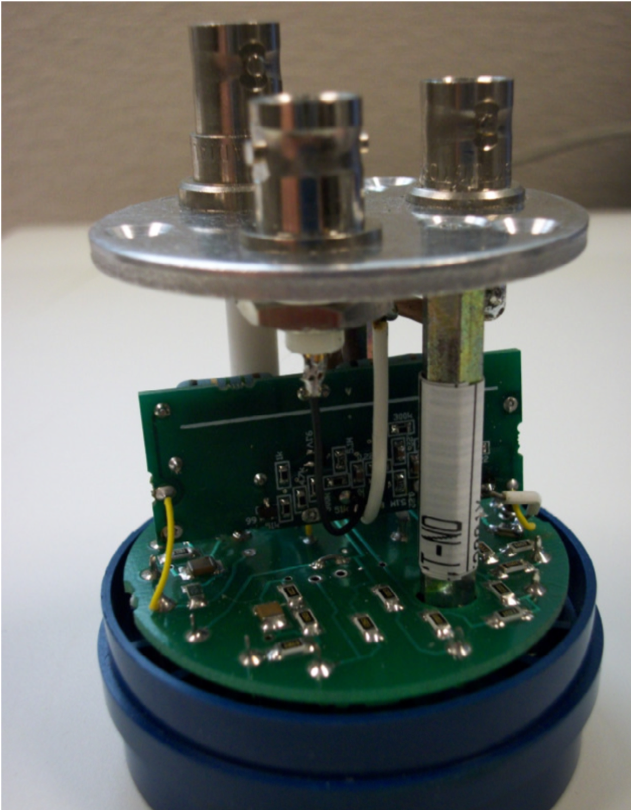
\includegraphics[width=0.95\columnwidth,keepaspectratio]{img/pmtWithDivider.png}
	\caption{The prototype module installed in the XP4500B PMT base. The bottom of the base has been modified to contain the HV
				BNC input and two output signals BNC. }
	\label{fig:pmtWithDivider}
\end{figure}

The following tests were performed successfully:
\begin{itemize}
	\item x10 amplification
	\item splitted signals identity
	\item signal to noise ratio comparison with non modified base
	\item FADC spectrum
\end{itemize}

In \F{dividerTests} (top) an empirical comparison of the two signals shows the similarity between the two output.
During testing of the modified PMT bases, the output has been processed by a Flash ADC electronic and acquired with a data
acquisition software using the PMT itself as trigger.
The corresponding SPE spectrum has been analyzed. The shape of the SPE signal is very similar to the original signal
coming from the external dedicated splitter and amplifier through the ADC electronics, see  \F{dividerTests} (bottom).

\begin{figure}
	\centering
	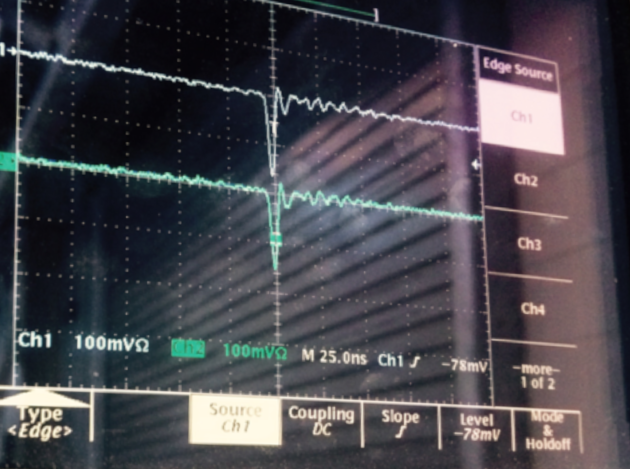
\includegraphics[width=0.87\columnwidth,keepaspectratio]{img/doubleSignal.png}
	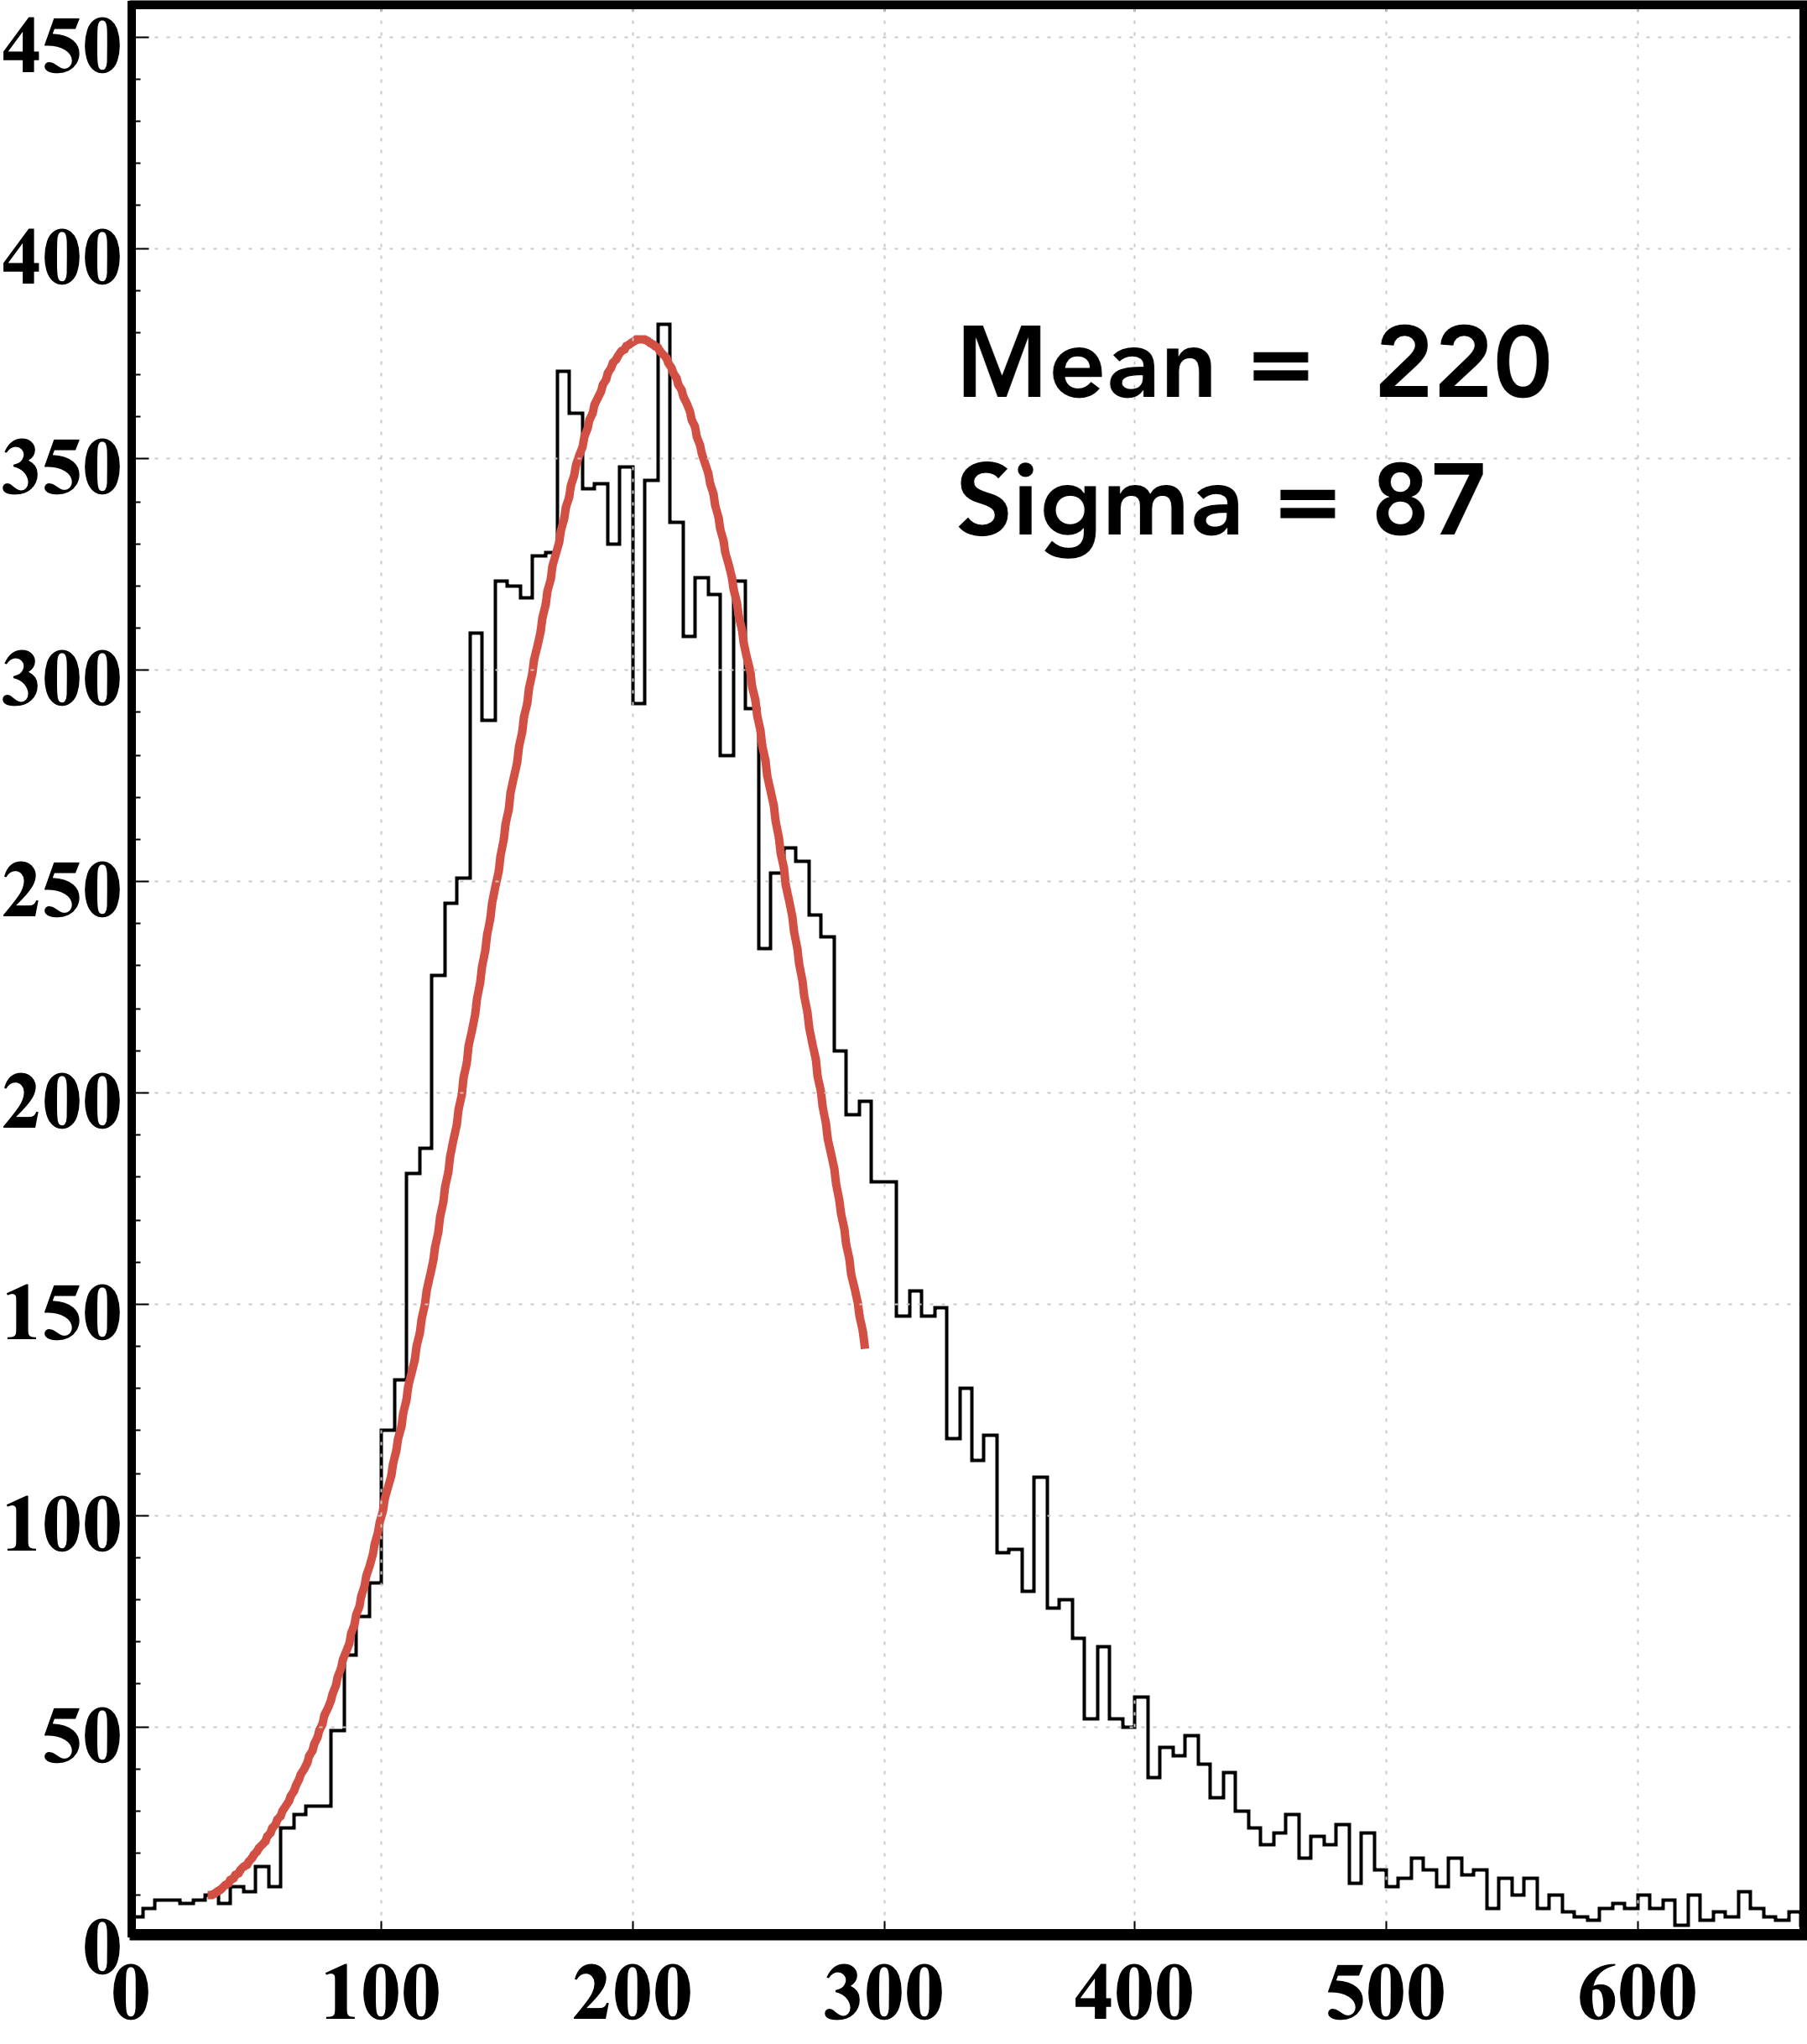
\includegraphics[width=0.97\columnwidth,keepaspectratio]{img/fadcOutput.png}
	\caption{Top: qualitetively comparison of the two outputs from the base modifications as seen on an oscilloscope.
				The analysis of the adc spectra histograms confirmed quantitevily that the signals are identical. Bottom:
				The single photo-electron ADC spectrum of one of the output compared with the PMT output in the original
            configuration of a dedicated external splitter and amplifier.
    }
	\label{fig:dividerTests}
\end{figure}

180 bases assembled at Jefferson Lab and installed on the PMT dividers. Both signals from all the modified bases were tested.
The response of the PMTs to the SPE resulted identical to the original output after it was amplified by a factor of 10, with one
clear advantage: the new bases allowed the PMTs to run at a HV average of 360 Volts less, see \F{pmtHVImprovement}.



\begin{figure}
	\centering
	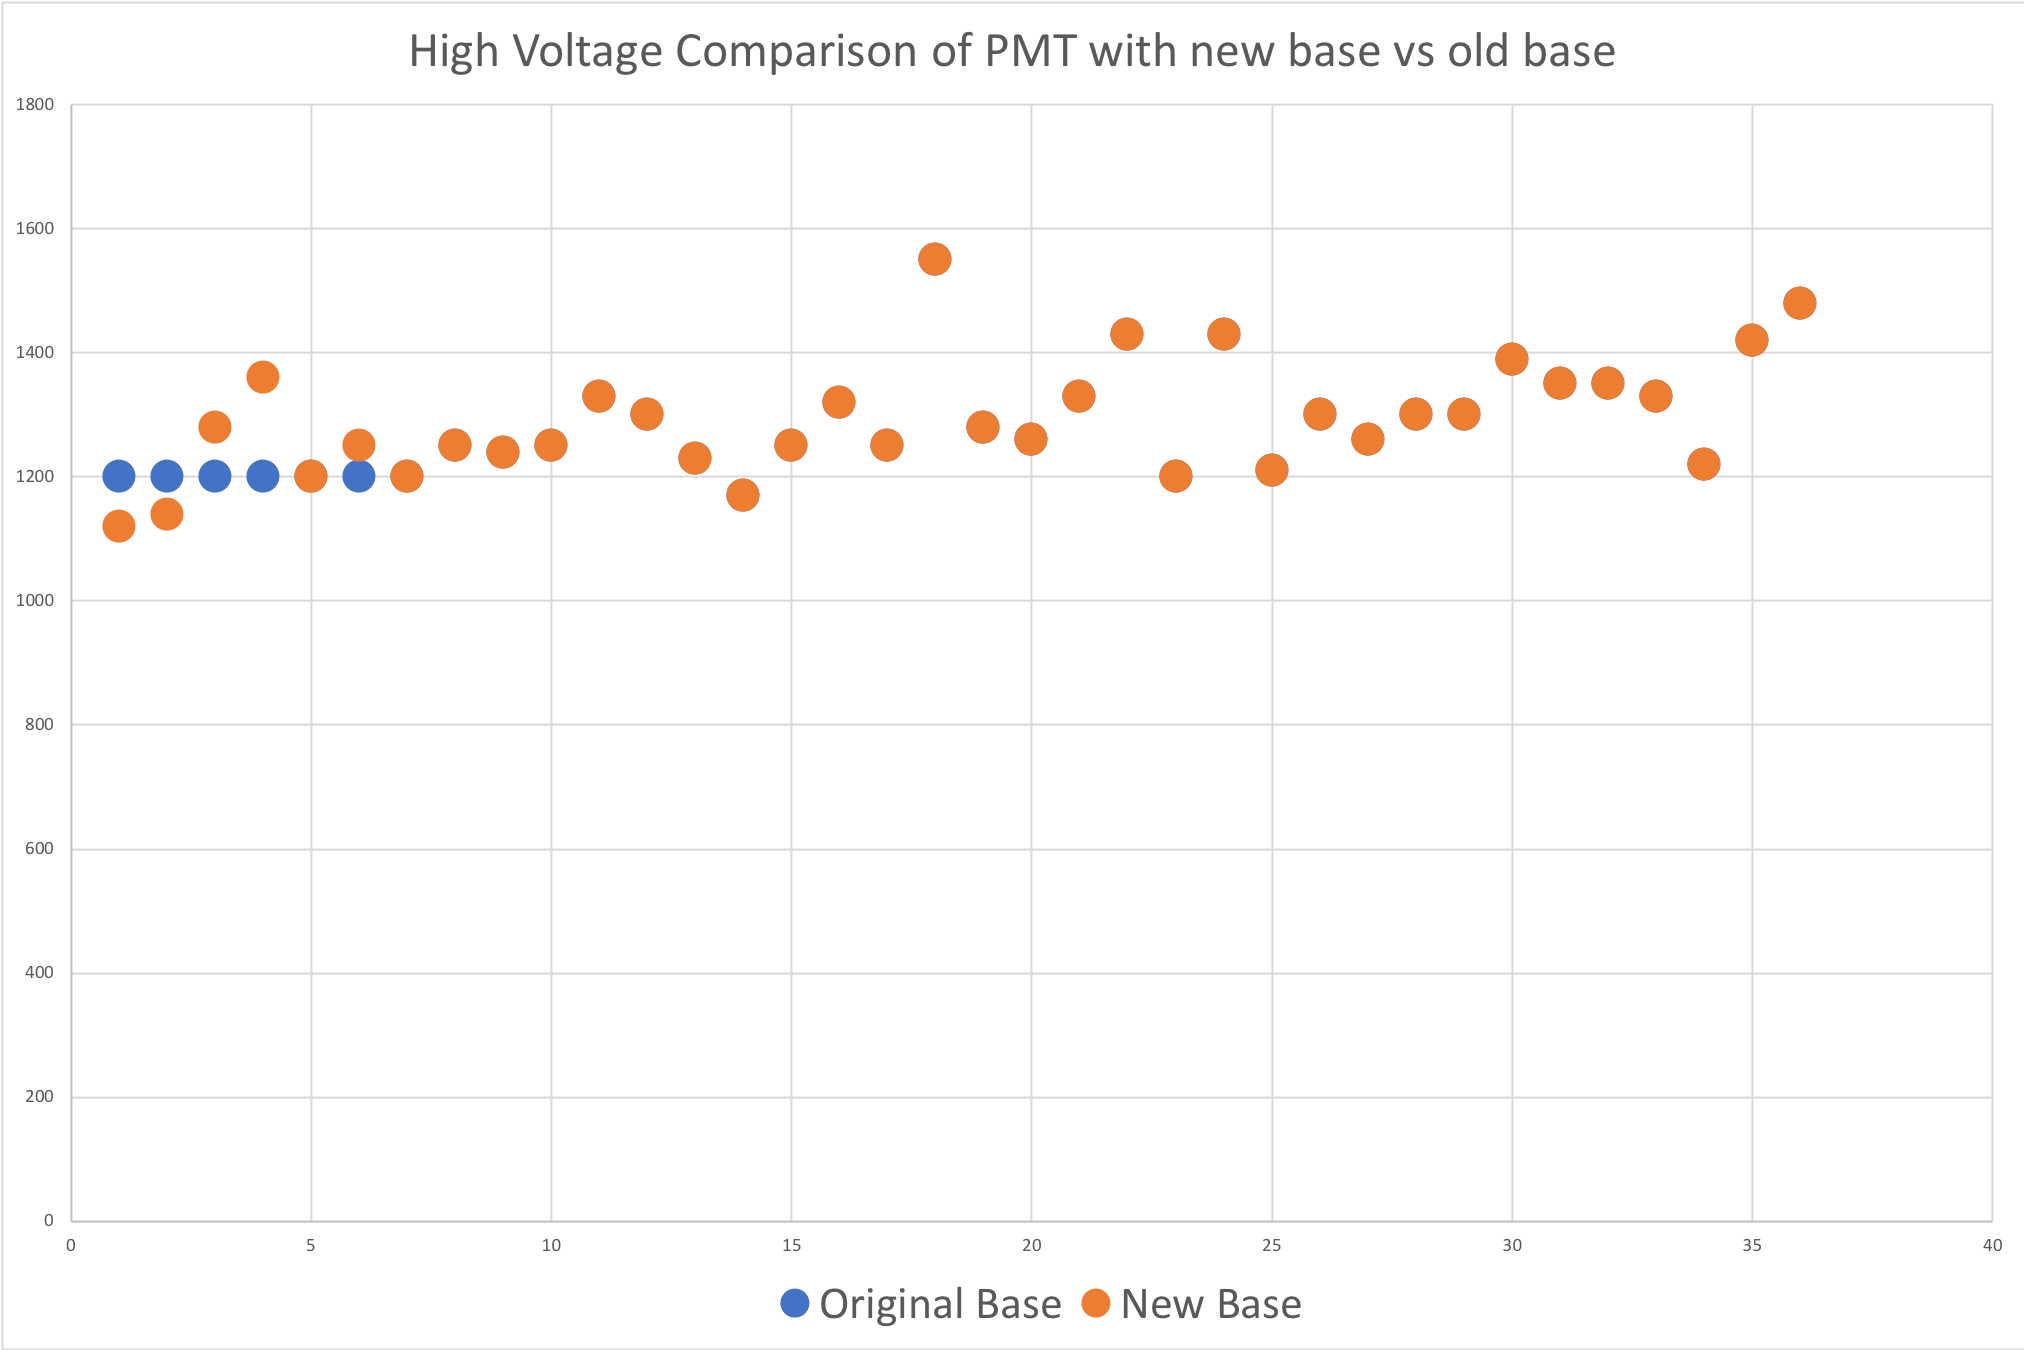
\includegraphics[width=0.95\columnwidth,keepaspectratio]{img/pmtHVImprovement.png}
	\caption{Comparison of sector 5 gain matched PMT high voltages that provide a SPE peak at about ADC channel 200.
            The PMTs with the modified bases could produce the same response function of the original base but at about 360 HV less voltage (1666 V vs 1292 V)}
	\label{fig:pmtHVImprovement}
\end{figure}
